%!TEX root = curso_EDA_SLIDES.tex


\section{Recursão}


\begin{frame}
\begin{center}
{\Large Capítulo 06 -- Recursão}
\end{center}

\begin{columns}
\begin{column}{.4\textwidth}
\centering
Pontos fundamentais a serem cobertos:
  \begin{enumerate}
  \item Contexto e motivação
  \item Definição
  \item Implementações
  \item Exercícios 
\end{enumerate}  
\end{column}

\begin{column}{.6\textwidth}
\centering
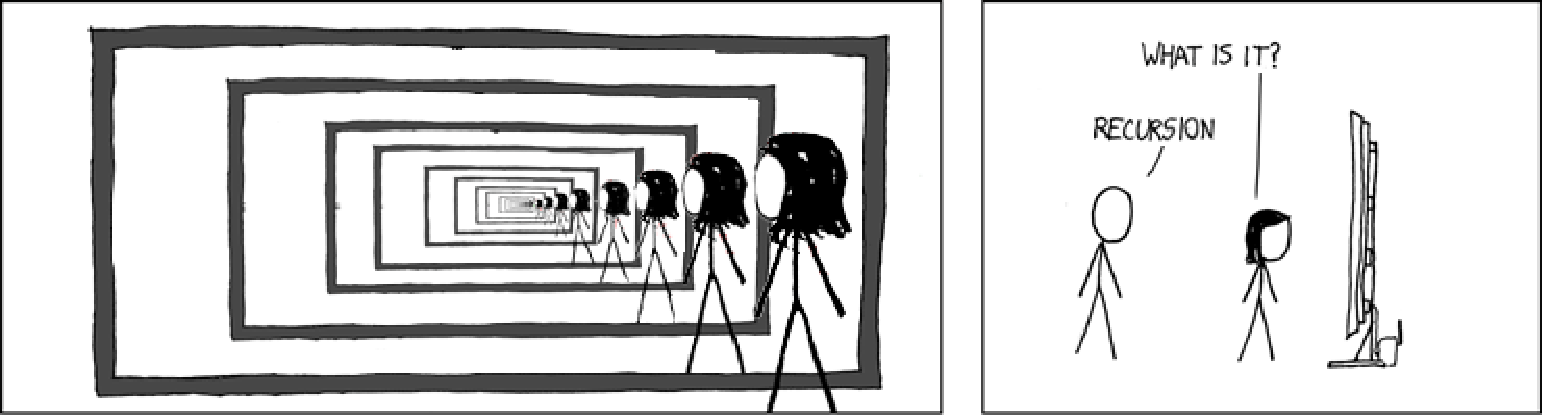
\includegraphics[height=4cm, width=7cm]{figs/fig_recursao/cartoon_recursao01.pdf}
%\hspace{+0.25cm}
%\scriptsize\textcolor{red}{[Tizio, Caio et al., Nature (2006)]}
\end{column}

\end{columns}


\end{frame}
%-----------------------------------------------------------------------

%--------------------

\begin{frame}[fragile]{Recursão}
\begin{itemize}
	\item Um objeto é dito recursivo se ele consistir parcialmente ou for definido em termos de si próprio. Recursões não são encontradas apenas em matemática mas também no dia a dia. 
	\item Recursão é uma técnica particularmente poderosa em definições matemáticas. Alguns exemplos: números naturais, estrutura de árvore e certas funções:
	
\begin{enumerate}
	\item Números naturais:	
		\begin{enumerate}
			\item 0 é um número natural.
			\item O sucessor de um número natural é um número natural.
		\end{enumerate}
	\item Estruturas de árvores	
		\begin{enumerate}
			\item 0 é uma árvore (chamada árvore vazia).
			\item Se $t_1$ e $t_2$ são árvores, então a estrutura que consiste de um nó com dois ramos $t_1 \ e \ t_2$ também é uma arvore.			
		\end{enumerate}
	\item A função fatorial $n!$
	
\begin{enumerate}
	\item 0! = 1
	\item $n > 0, n! = n * (n - 1)$
\end{enumerate}
\end{enumerate}
\end{itemize}
\end{frame}  

\begin{frame}[fragile]{Recursão}
\begin{itemize}
	\item Se uma função $f$ possuir uma referência explícita a si próprio, então a função é dita \textit{diretamente recursiva}. Se $f$ contiver uma referência a outra função $g$, que por sua vez contém uma referência direta ou indireta a $f$, então $f$ é dita \textit{indiretamente recursiva}.
	\item Em termos matemáticos, a recursão é uma técnica que através de substituições sucessivas reduz o problema a ser resolvido a um caso de solução mais simples (Dividir para conquistar).
\end{itemize}
\end{frame}


\begin{frame}[fragile]{Recursão}
\framesubtitle{Exemplo}
\footnotesize
\begin{lstlisting}[language=C]
/**
 * Calcula a soma dos numeros inteiros 
 * existentes entre in e n inclusive.
 */
int somatorio(int in, int n){   
 int s = in;
 if (s < n)
 {      
   return s + somatorio(s + 1, n);
 }
 return s;
}

public static void main(String args)
{    
   print(somatorio(1, 100));
}
\end{lstlisting}
\end{frame}


\begin{frame}[fragile]{Recursão}
\begin{enumerate}
	\item Há dois requisitos-chave para garantir que a recursão tenha sucesso:	
			\begin{enumerate}
				\item Toda chamada recursiva tem de simplificar os cálculos de alguma maneira.
				\item Tem de haver casos especiais para tratar os cálculos mais simples diretamente.
			\end{enumerate}
	\item Muitas recursões podem ser calculadas com laços. Entretanto, as soluções iterativas para problemas recursivos podem ser mais complexas.
	\item Por exemplo, a permutação de uma palavra.
\end{enumerate}
\end{frame}

\begin{frame}[fragile]{Recursão}
\begin{itemize}
	\item A permutação é um exemplo de recursão que seria difícil de programar utilizando laços simples.
	\item Uma permutação de uma palavra é simplesmente um rearranjo das letras. Por exemplo, a palavra ``eat'' tem seis permutações ($n!$, onde $n$ é o número de letras que formam a palavra).
	\item Como gerar essas permutações?
	\item Simples, primeiro, gere todas as permutações que iniciam com a letra ``e'', depois as que iniciam com a letra ``a'' e finalmente as que iniciam com a letra ``t''.
	\item Mas, como gerar as permutações que iniciam com a letra ``e''?
	\item Gere as permutações da sub-palavra ``at''. Porém, esse é o mesmo problema, mas com uma entrada mais simples, ou seja, uma palavra menor.
	\item Logo, podemos usar a recursão nesse caso.
\end{itemize}
\end{frame}


\begin{frame}[fragile]{Recursão}
\begin{block}{Como pensar recursivo}  
		\begin{enumerate}
			\item Combine várias maneiras de simplificar as entradas.
			\item Combine as soluções de entradas mais simples para uma solução do problema original.
			\item Encontre soluções para as entradas mais simples.
			\item Implemente a solução combinando os casos simples e o passo de redução.
		\end{enumerate}
\end{block}
\end{frame}

\begin{frame}[fragile]{Eficiência da Recursão}
\begin{enumerate}
	\item A recursão pode ser uma ferramenta poderosa para implementar algoritmos complexos.
	\item No entanto, a recursão pode levar a algoritmos que tem um desempenho fraco.
	\item Vejamos quando a recursão é benéfica e quando é ineficiente.	
\end{enumerate}
\end{frame}

\begin{frame}[fragile]{Eficiência da Recursão}
\begin{enumerate}
	\item Considere a sequência de Fibonacci, uma sequência de números inteiros definidos pela equação:
	$$f_1 = 1$$
	$$f_2 = 1$$
	$$f_n = f_{n - 1} + f_{n - 2}$$
	\item Exemplo: $1,1,2,3,5,8,13,21,34,55, \ \cdots$.
	\item Vejamos uma implementação recursiva que calcule qualquer valor de $n$.	
\end{enumerate}
\end{frame}

\begin{frame}[fragile]{Eficiência da Recursão}
% \tiny{
\begin{lstlisting}[language=C]

  int fibonacci(int n) {				
    if (n <= 2)
      return 1;
    else
      return fibonacci(n - 1) + fibonacci(n - 2);		
  }

  void main(void) {
    int i;
    for (i = 1; i <= n; i++) {
      int f = fibonacci(i);
      printf("%d",  f);
    }
  }
}
\end{lstlisting}
% }
\end{frame}

\begin{frame}[fragile]{Eficiência da Recursão}

\begin{enumerate}
	\item Ao executarmos o programa de teste podemos notar que as primeiras chamadas à função \textbf{fibonacci} são bem rápidas. No entanto, para valores maiores, o programa pausa um tempo considerável entre as saídas.
	\item Inicialmente isso não faz sentido, uma vez que podemos calcular de forma rápida com auxílio de uma calculadora esses números, de modo que para o computador não deveria demorar tanto em hipótese alguma.
	\item Para descobrir o problema, vamos inserir mensagens de monitoração das funções e verificar a execução para $n = 6$.
\end{enumerate}
\end{frame}

\begin{frame}[fragile]{Eficiência da Recursão}
\tiny{
Início fibonacci n = 6\\
Início fibonacci n = 5\\
Início fibonacci n = 4\\
Início fibonacci n = 3\\
Início fibonacci n = 2\\
Término fibonacci n = 2, retorno = 1\\
Início fibonacci n = 1\\
Término fibonacci n = 1, retorno = 1\\
Término fibonacci n = 3, retorno = 2\\
Início fibonacci n = 2\\
Término fibonacci n = 2,\ retorno = 1\\
Término fibonacci n = 4, retorno = 3\\
Início fibonacci n = 3\\
Início fibonacci n = 2\\
Término fibonacci n = 2, retorno = 1\\
Início fibonacci n = 1\\
Término fibonacci n = 1, retorno = 1\\
Término fibonacci n = 3, retorno = 2\\
Término fibonacci n = 5, retorno = 5\\
Início fibonacci n = 4\\
Início fibonacci n = 3\\
Início fibonacci n = 2\\
Término fibonacci n = 2, retorno = 1\\
Início fibonacci n = 1\\
Término fibonacci n = 1, retorno = 1\\
Término fibonacci n = 3, retorno = 2\\
Início fibonacci n = 2\\
Término fibonacci n = 2, retorno = 1\\
Término fibonacci n = 4, retorno = 3\\
Término fibonacci n = 6, retorno = 8\\
Fibonacci(6) = 8\\
}
\end{frame}


\begin{frame}[fragile,plain]{Eficiência da Recursão}
\Tree [.f(6) [.f(5) [.f(4) [.f(3) f(2) f(1) ] f(2) ] [.f(3) f(2) f(1) ] ] [.f(4) [.f(3) f(2) f(1) ] f(2) ] ] 

\begin{center} Padrão de chamada de função/método recursivo \textit{fibonacci}. \end{center}
\end{frame}

\begin{frame}[fragile,plain]{Eficiência da Recursão}
\begin{enumerate}
	\item Analisando o rastro de execução do programa fica claro porque o método leva tanto tempo. 
	\item Ele calcula os mesmos valores repetidas vezes.
	\item Pelo exemplo, o calculo de \textbf{fibonacci(6)} chama \textbf{fibonacci(4)} duas vezes, \textbf{fibonacci(3)} três vezes, \textbf{fibonacci(2)} cinco vezes, e \textbf{fibonacci(1)} três vezes. 
	\item Diferente do cálculo que faríamos manualmente.
\end{enumerate}

\Tree [.f(6) [.f(5) [.\textcolor{red}{f(4)} [.\textcolor{blue}{f(3)} \textcolor{green}{f(2)} f(1) ] \textcolor{green}{f(2)} ] [.\textcolor{blue}{f(3)} \textcolor{green}{f(2)} f(1) ] ] [.\textcolor{red}{f(4)} [.\textcolor{blue}{f(3)} \textcolor{green}{f(2)} f(1) ] \textcolor{green}{f(2)} ] ] 
\end{frame}

\begin{frame}[fragile,plain]{Em resumo...}
\begin{block}{Eficiência da Recursão}
As vezes acontece de uma solução recursiva ser executada muito mais lentamente do que sua equivalente iterativa. Entretanto, na maioria dos casos, a solução recursiva é apenas levemente mais lenta.
\end{block}
\begin{block}{}
Em muitos casos, uma solução recursiva é mais fácil de entender e implementar corretamente do que uma solução iterativa.
\end{block}
\end{frame}
